\documentclass{article}
\usepackage{float}
\usepackage{graphicx}
\graphicspath{{images/}}

\newcommand{\changefont}{%
	\fontsize{9}{11}\selectfont
}
\newcommand*{\TitleFont}{%
	\usefont{\encodingdefault}{\rmdefault}{b}{n}%
	\fontsize{40}{20}%
	\selectfont}

\newcommand*{\SubTitleFont}{%
	\usefont{\encodingdefault}{\rmdefault}{b}{n}%
	\fontsize{24}{20}%
	\selectfont}
\begin{document}
	\title{\TitleFont Test Cases For Monitoring}
	\date{2018-01-05}
	\author{\SubTitleFont Project Group 6\\}
	\maketitle
	\newpage

	
	\section*{Case 1:}

	Title: Access Home Page – Accesing Successfully on Devops Monitoring Home Page
	\newline
	Description: A registered user should be able to successfully access the Devops Monitoring.
	\newline
	Precondition: zabbix server should be up and running.
	\newline
	Assumption: having internet connection and  supported browser.
	\newline
	\newline
	Test Steps:
	\begin{itemize}
\item[1.] Navigate to any browser that you can gain access.
\item[2.]In the address bar write the address of the localhost. 
\item[3.]Click the ‘Enter’ button.
	\end{itemize}
	Expected Result: Devops Home Page opens:
	
	\begin{figure}[H]
		\centering
		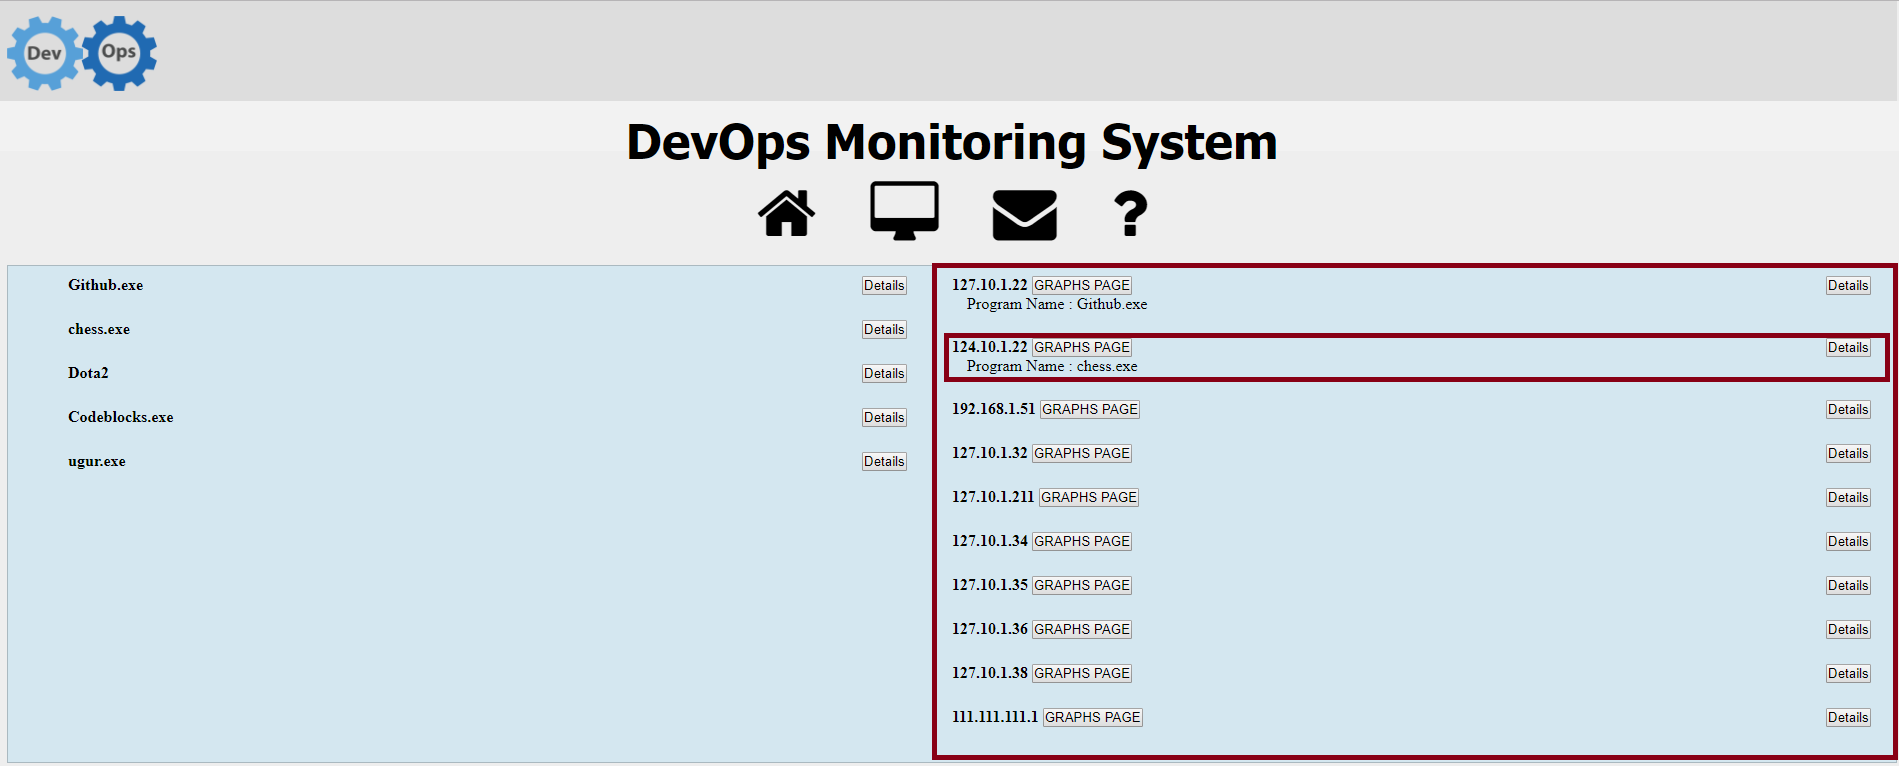
\includegraphics[scale=0.3,width=\linewidth]{1}
		\caption{Home Page}
	\end{figure}
	
	
\section*{Case 2:}
 	
		Title: Monitoring Programs In A Host  – Monitoring Executable Programs Which Are  Deployed  In A Host.
	\newline
	Description: A devops user should be able to successfully monitor all programs in a host.
	\newline
	Precondition: zabbix server should be up and running.
	\newline
	Assumption: Having internet connection, connetted to Monitoring home page and running Zabbix server.
	\newline
	\newline
	Test Steps:
	\begin{itemize}
		\item[1.] 	Click the “Details” button on the right side of the page for each host to see applications installed in it.
		\item[2.]	Click “GRAPH PAGE” button to view graphs of all the applications in a scpecific host.
		
	\end{itemize}
	Expected Result: DevOps users see links of all graphs in a host.
	
	\begin{figure}[H]
		\centering
		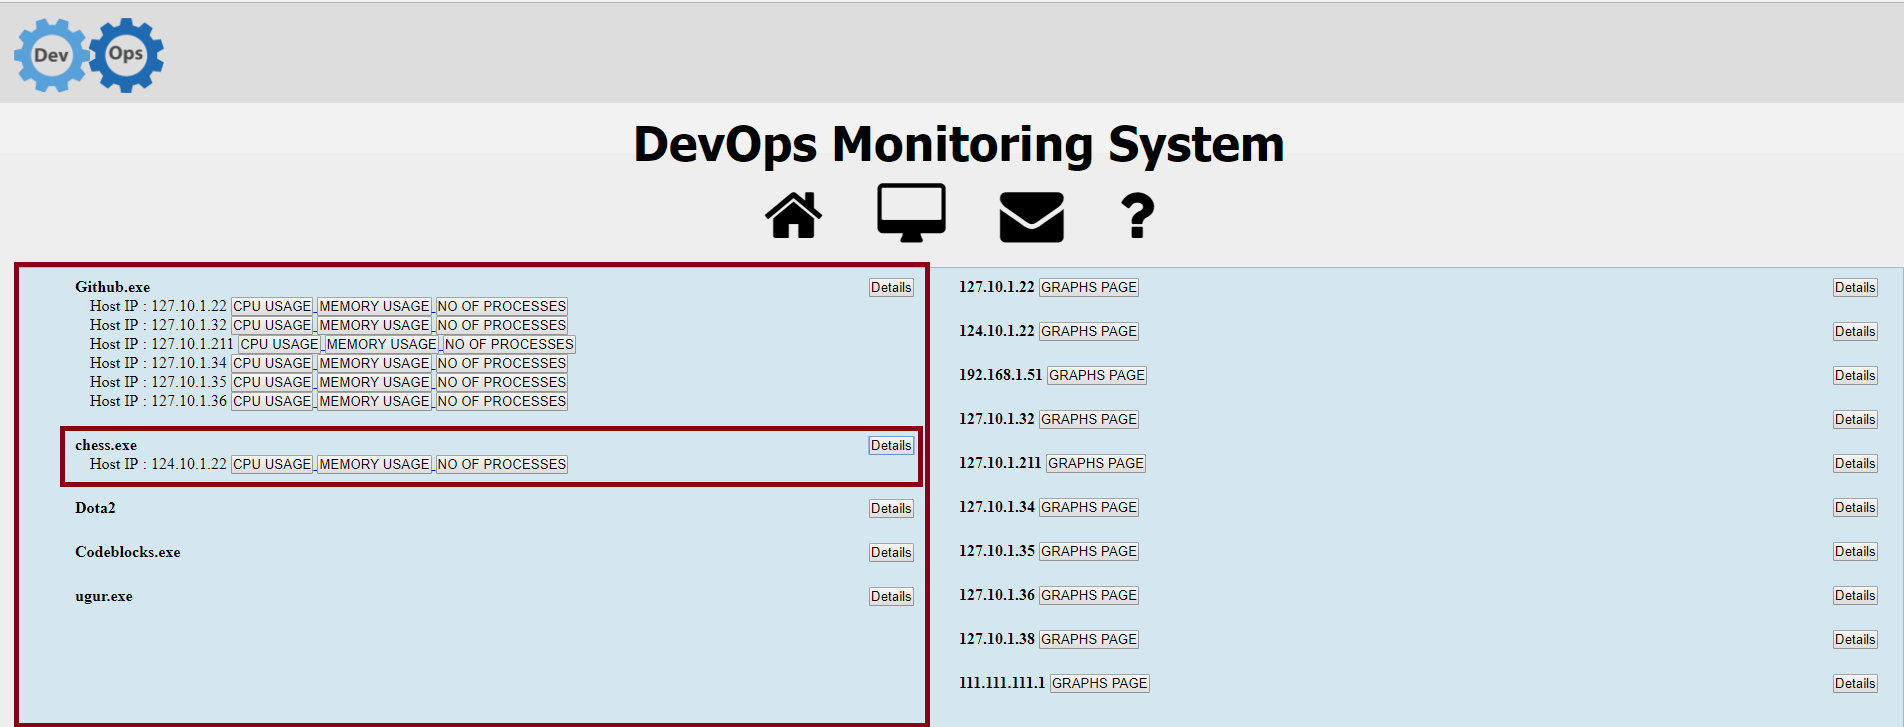
\includegraphics[scale=0.3,width=\linewidth]{2}
		\caption{Programs In a Host}
	\end{figure}
	
\section*{Case 3:}
	Title: Monitoring Program’s CPU Usage  – Monitoring CPU usage of An Executable Program Which Is Deployed To Hosts.
		\newline
	Description: A devops user should be able to successfully monitor CPU usage of a program in every host it is deployed.
	\newline
	Precondition: Zabbix server should be up and running.
	\newline
	Assumption:  If a program is installed in at least one host, having Internet connection, connected to Monitoring home page and running Zabbix server.
	\newline
	\newline
	Test Steps:
	\begin{itemize}
	\item[1.]	Click the “Details” button on the left side of the page for each program.
	\item [2.]	Click the “CPU USAGE” button that you want to view.
	\end{itemize}
	Expected Result: DevOps users can see a graph with CPU usage information of an application in a desired host.
	
		\begin{figure}[H]
		\centering
		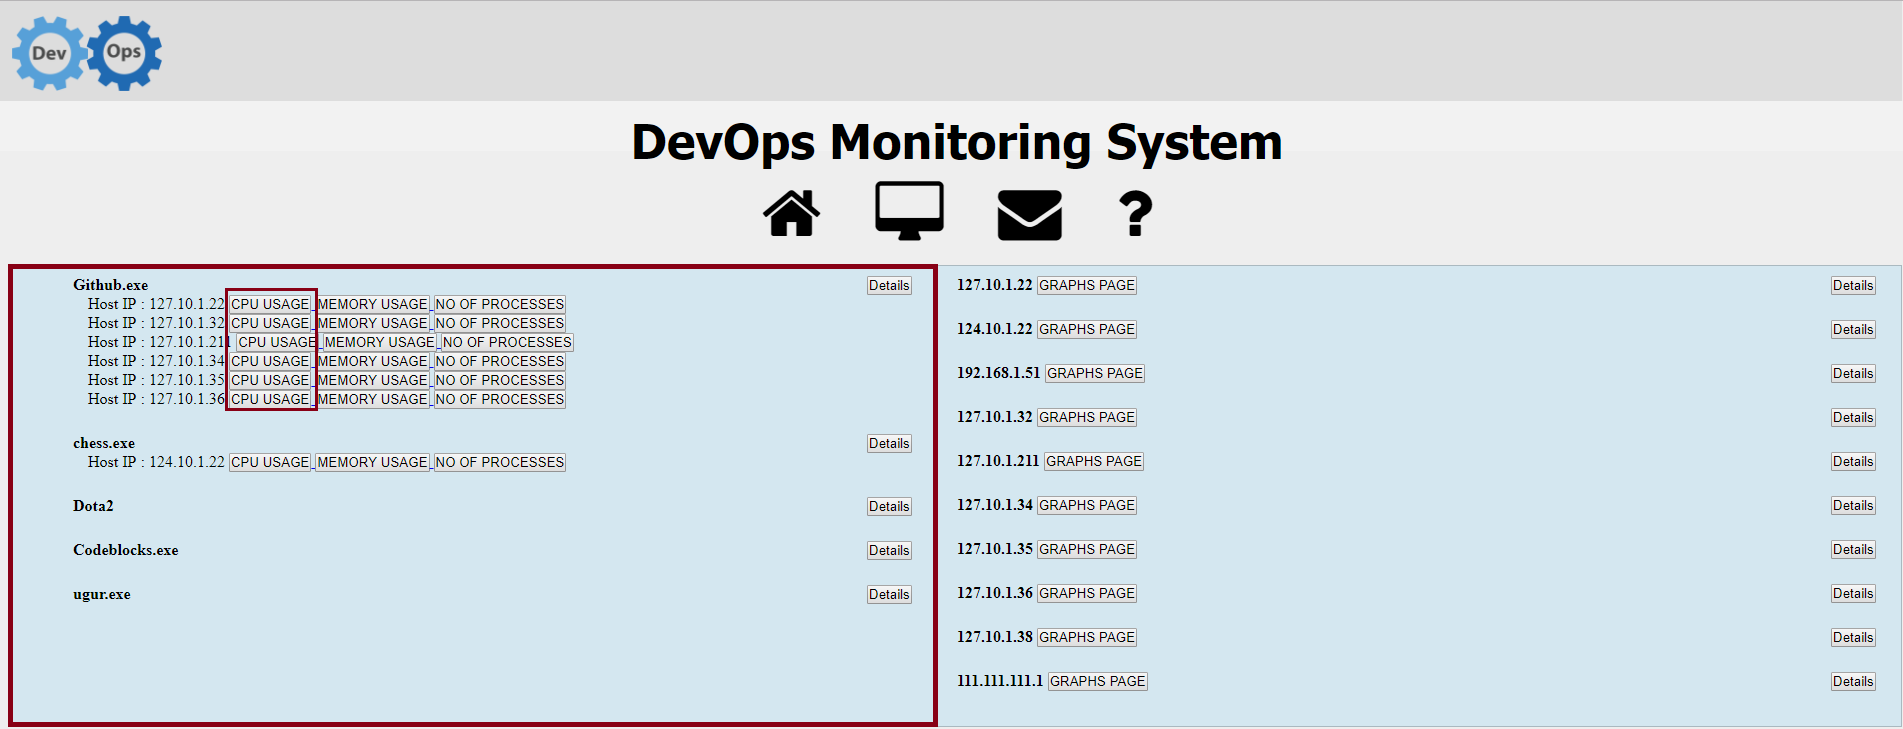
\includegraphics[scale=0.4,width=\linewidth]{3}
		\caption{CPU usage}
	\end{figure}
	
	\section*{Case 4:}
	Title: Monitoring Program’s Memory Usage  – Monitoring Memory Usage Of An Executable Program Which Is Deployed To Hosts.
	\newline
	Description: A devops user should be able to successfully monitor memory usage of a program in  host which he/she want to monitor.
	\newline
	Precondition: Zabbix server should be up and running.
	\newline
	Assumption:  If a program is installed in at least one host, having internet connection, connected to Monitoring home page and running Zabbix server.
	\newline
	\newline
	Test Steps:
	\begin{itemize}
	
	
	\item[1.]Click the “Details” button on the left side of the page for each program.
	\item[2.]Click the “MEMORY USAGE” button that you want to view.
	\end{itemize}
	Expected Result: DevOps users can see graph information of memory usage of an application in a specific host.
	
		\begin{figure}[H]
		\centering
		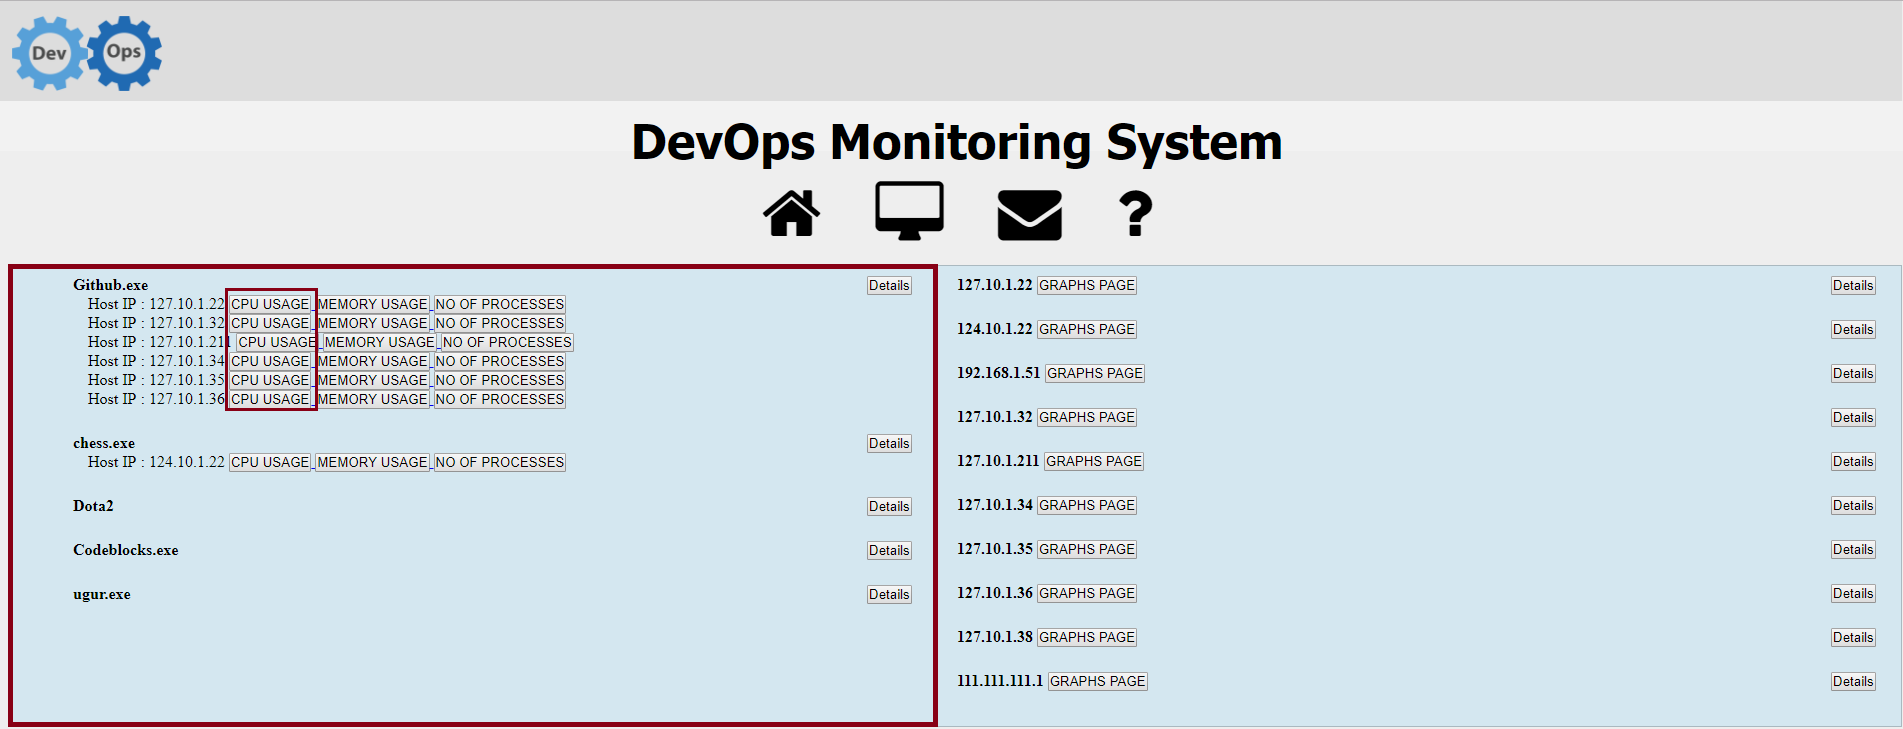
\includegraphics[scale=0.4,width=\linewidth]{3}
		\caption{Memory Usage}
	\end{figure}
	\section*{Case 5:}
	Title: Monitoring Program’s Number of Processes  – Monitoring Number of processes of an application in a specific host.
	\newline
	Description: A devops user should be able to successfully monitor number of processes of program in  host which he/she want to monitor.
	\newline
		Precondition: Zabbix server should be up and running.
	\newline
	Assumption:  If a program is installed in at least one host, having internet connection, connected to Monitoring home page and running Zabbix server.
	\newline
	\newline
	Test Steps:
	\begin{itemize}
	

	\item[1.]Click the “Details” button on the left side of the page for each program.
	\item[2.]Click the “NO OF PROCESSES” button that you want to view.
	\end{itemize}
	Expected Result: DevOps users can see a graph with process information of an application in a desired host.
	
		\begin{figure}[H]
		\centering
		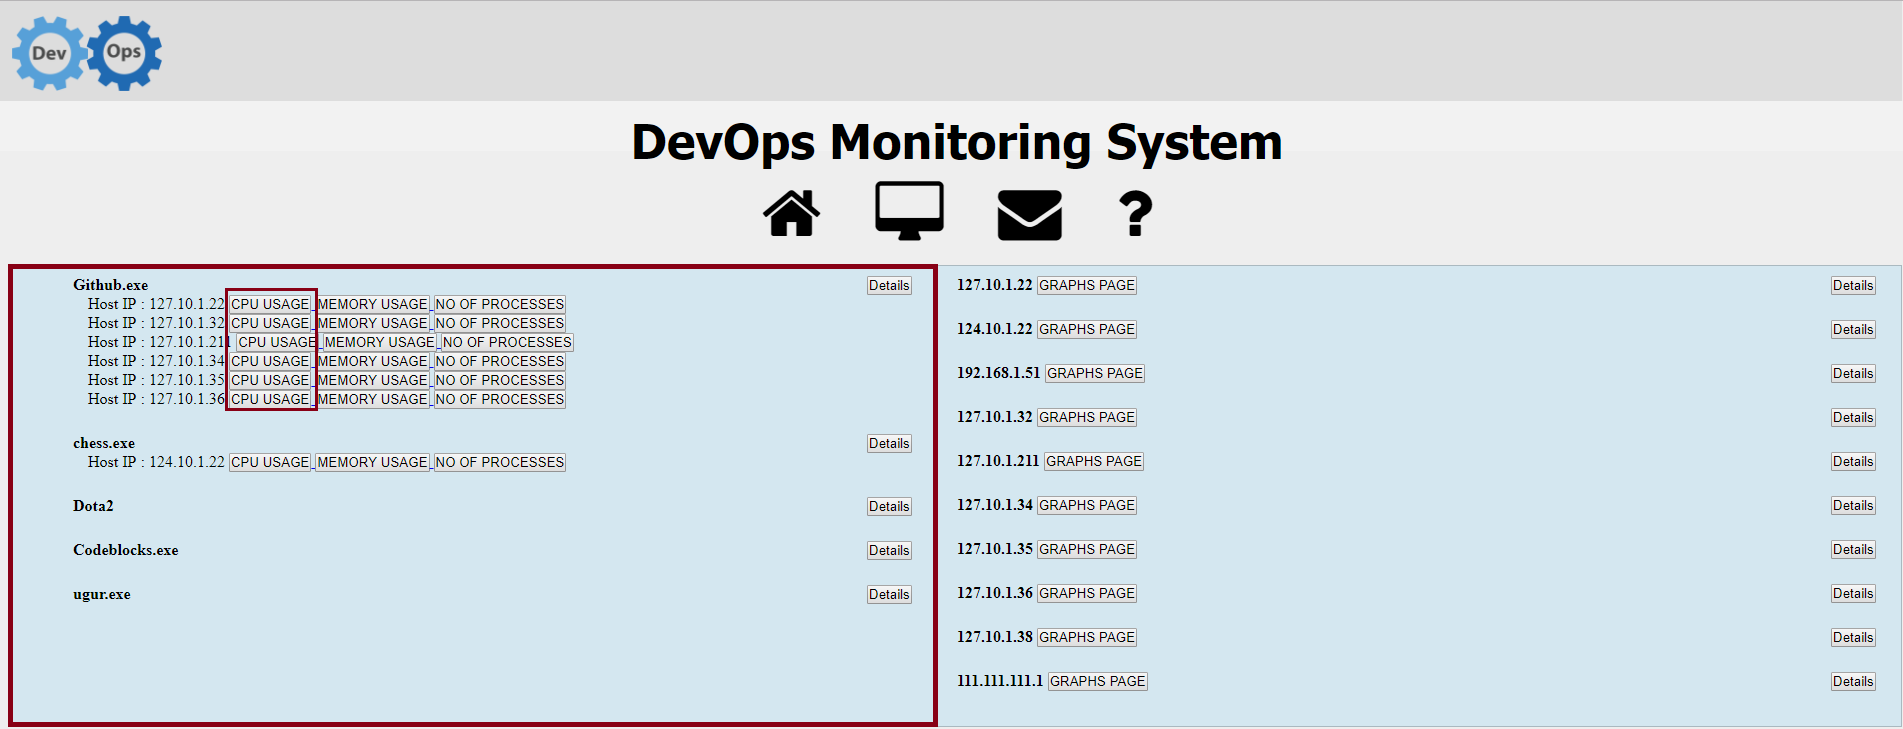
\includegraphics[width=\linewidth]{3}
		\caption{Number Of Processes}
	\end{figure}
	
	
	
\end{document}